\documentclass[10pt, a4paper]{report}

\usepackage[utf8]{inputenc}
\usepackage{polski}
\usepackage{a4wide}
\usepackage{fancyhdr}
\usepackage{lastpage}
\usepackage{tabularx}
\usepackage{graphicx}

\graphicspath{ {./images} }

%strona tytułowa
\begin{titlepage}

\title{\huge{\textbf{Sprawozdanie}} \\ programu aprox}
\author{Szymon Półtorak i Sebastian Sikorski}
\date{}

\end{titlepage}

\renewcommand{\footrulewidth}{1pt}

\begin{document}
    \maketitle

    \renewcommand*\thesection{\arabic{section}} 
    
    \pagestyle{fancy}
    \fancyhf{}
    \rhead{Szymon Półtorak i Sebastian Sikorski}
    \cfoot{Strona \thepage \hspace{1pt} z \pageref{LastPage}}
    
    \fancypagestyle{plain}{
        \rhead{Szymon Półtorak i Sebastian Sikorski}
        \cfoot{Strona \thepage \hspace{1pt} z \pageref{LastPage}}
    }
    \tableofcontents
    \newpage

    \section{Opis teoretyczny zagadnienia}
    \textbf{Wielomiany Hermite’a} – wielomiany o współczynnikach rzeczywistych, będące rozwiązaniem równania rekurencyjnego 
    \begin{figure}[h]
        \begin{center}
            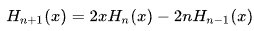
\includegraphics[scale=0.8]{hermit1.jpg}
            \caption{Wzór rekurencyjny}
        \end{center}
    \end{figure}

    \begin{figure}[h]
        \begin{center}
            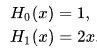
\includegraphics[scale=0.8]{hermit2.jpg}
            \caption{Warunki początkowe}
        \end{center}
    \end{figure}

    Pierwszy z tych wzorów bywa nazywany wzorem Rodrigueza:
    \begin{figure}[h]
        \begin{center}
            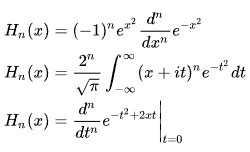
\includegraphics[scale=0.8]{hermit3.jpg}
            \caption{Wzory wielomianów Hermite'a}
        \end{center}
    \end{figure}
    Wykresy czterech pierwszych wielomianów oraz wzory pierwszych siedmiu:
    \begin{figure}[h]
        \begin{center}
            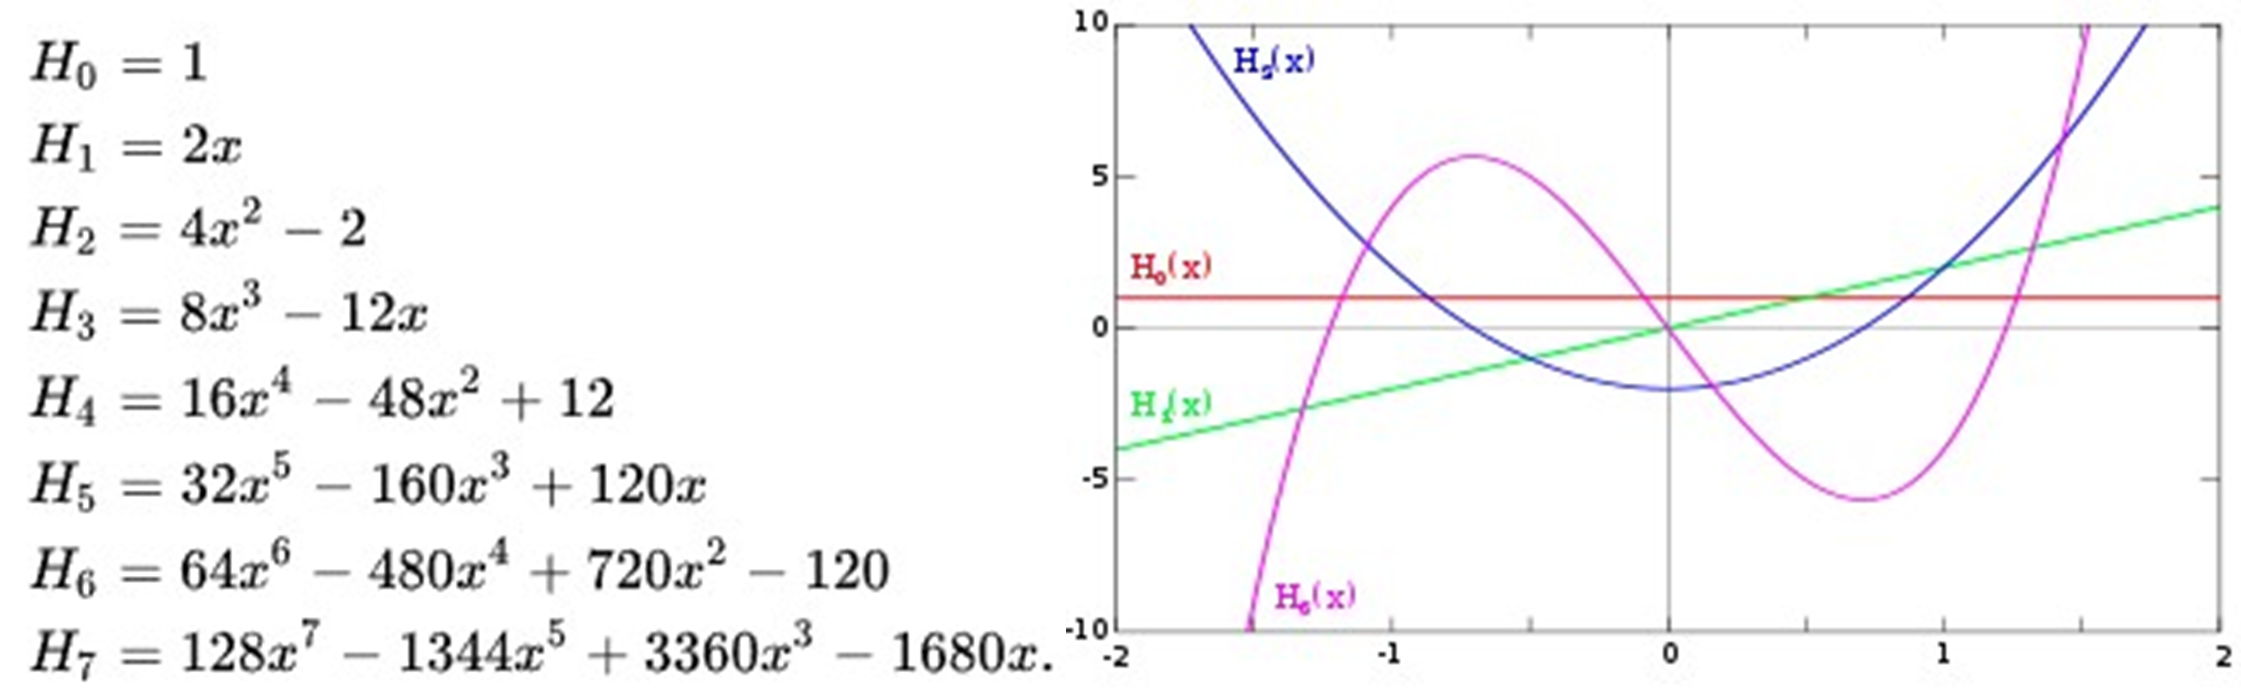
\includegraphics[scale=0.8]{hermit4.png}
            \caption{Wykresy pierwszych czterech wielomianów}
        \end{center}
    \end{figure}
    \newpage

    \section{Opis wywołania programu}
    Aby skompilować program wystarczyć użyć komendy „make”. Zostaną utworzone wszystkie pliki wykonywalne.
    \begin{figure}[h]
        \begin{center}
            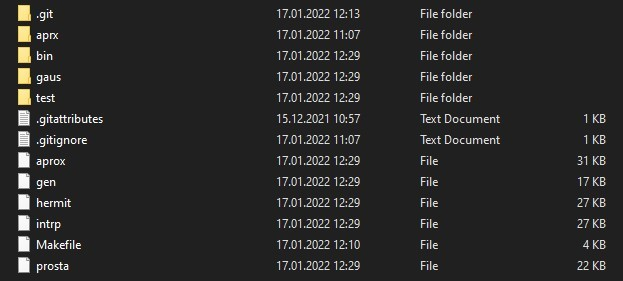
\includegraphics[scale=0.8]{run1.jpg}
            \caption{Utworzone pliki aprox gen hermit intrp i prosta }
        \end{center}
    \end{figure}

    Pliki:
    \begin{itemize}
        \item gen – odpowiada za generowanie „losowe” danych,
        \item aprox – program zajmujący się aproksymacją,
        \item hermit – aproksymacja na bazie wielomianów Hermite’a,
        \item intrp – interpolator na bazie wielomianów Lagrange’a,
        \item prosta – dopasowuje do punktów prostą najlepszego dopasowania,
    \end{itemize}
    Wpisując \texttt{./<wybrany program>} wyświetli się instrukcja jego wywołania. 
    \begin{figure}[h]
        \begin{center}
            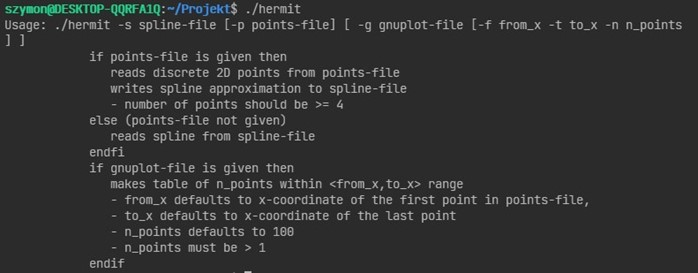
\includegraphics[scale=0.8]{run2.jpg}
            \caption{Wywołanie bez argumentów}
        \end{center}
    \end{figure}
    \newpage

    Wywołanie: 
    \newline\texttt{./hermit -s spl -p test/dane.1 -g myplot -f 5.1 -t 5.7 -n 300} 
    \newline\newline Następnie trzeba otworzyć program rysujący funkcję przykładowo gnuplota i użyć komendy plot np.  plot ‘test/dane.1’, ‘myplot’ 
    \newline
    \begin{figure}[h]
        \begin{center}
            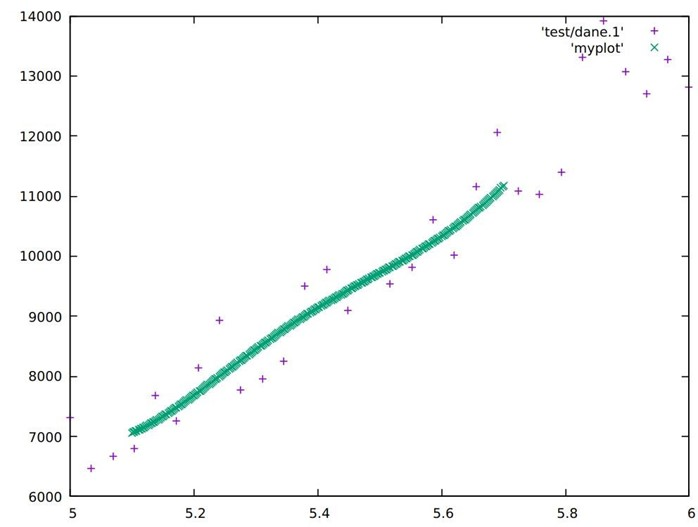
\includegraphics[scale=0.6]{run3.jpg}
            \caption{Przykładowy wynik aproksymacji}
        \end{center}
    \end{figure}

    \section{Testy dla różnych zestawów wejściowych}
    Po użyciu komendy make test\_hermit można zobaczyć 2 różne wykresy rysowane przez naszą funkcję.
    \begin{figure}[h]
        \begin{center}
            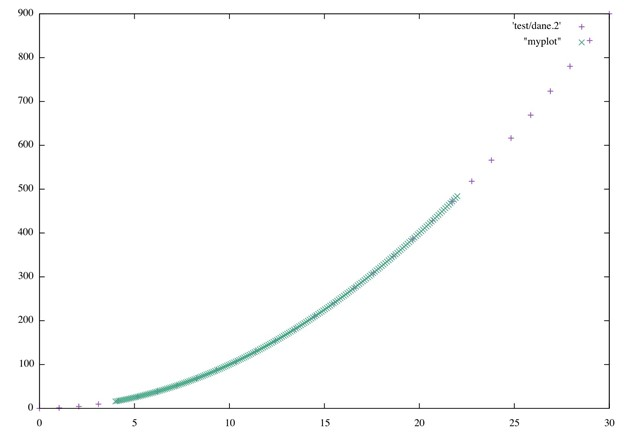
\includegraphics[scale=0.6]{test1.jpg}
            \caption{Dane testowe 1}
        \end{center}
    \end{figure}

    \begin{figure}[h]
        \begin{center}
            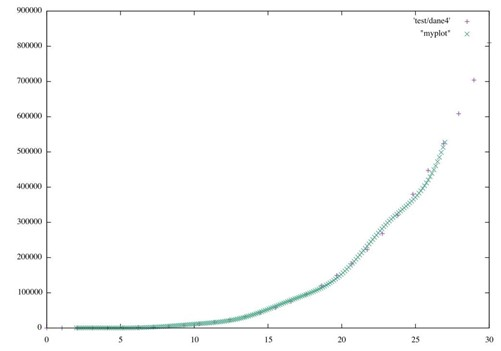
\includegraphics[scale=0.8]{test2.jpg}
            \caption{Dane testowe 2}
        \end{center}
    \end{figure}
    \newpage

    \section{Porównanie z działającą aproksymacją}
    \begin{figure}[h]
        \begin{center}
            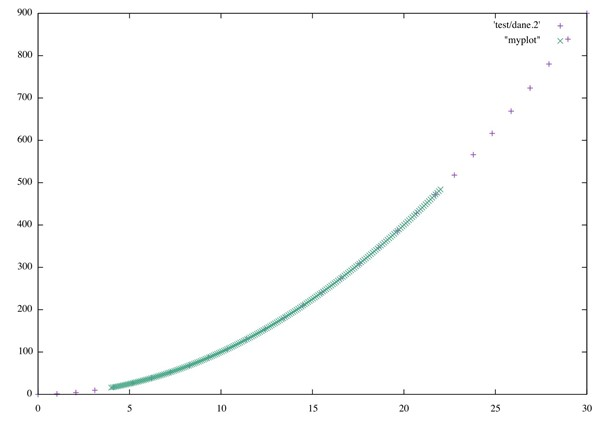
\includegraphics[scale=0.6]{compare1.jpg}
            \caption{Użycie wielomianów hermite'a}
        \end{center}
    \end{figure}

    \begin{figure}[h]
        \begin{center}
            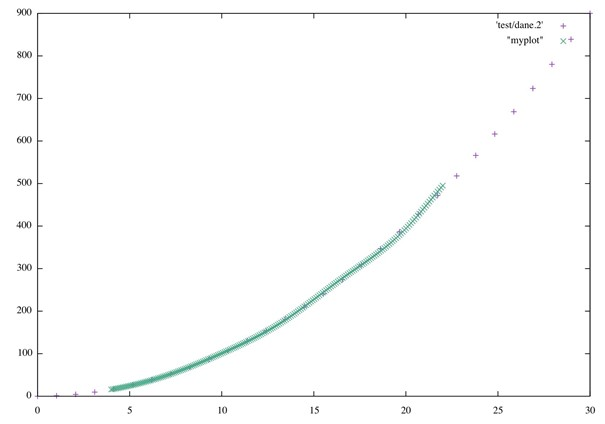
\includegraphics[scale=0.6]{compare2.jpg}
            \caption{Użycie zwykłej zaproksymacji}
        \end{center}
    \end{figure}
    \newpage

    \section{Wnioski}
    Wprowadzenie bazy wielomianów hermite’a działa prawidłowo, niektóre funkcje (przykład wyżej) otrzymują lepsze wyniki aproksymacji niż nawet ze standardowym programem ./aprox.

    \section{Błędy znalezione w programie i ich poprawa}
    Poprawiliśmy brak rzutowania podczas mallocowania wskaźników:
    \begin{figure}[h]
        \begin{center}
            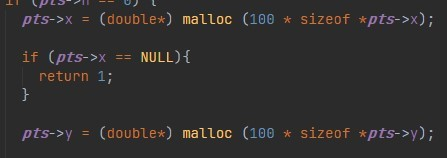
\includegraphics[scale=0.7]{error1.jpg}
            \caption{Użycie zwykłej zaproksymacji}
        \end{center}
    \end{figure}
    
    Dodaliśmy zamykanie plików w przypadku obsługi fclose:
    \begin{figure}[h]
        \begin{center}
            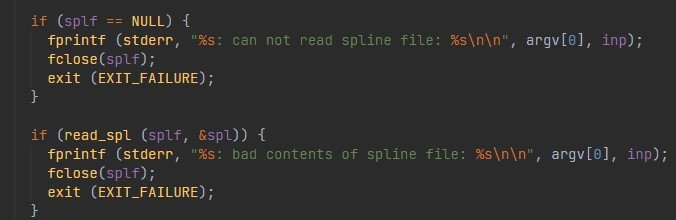
\includegraphics[scale=0.7]{error2.jpg}
            \caption{Użycie zwykłej zaproksymacji}
        \end{center}
    \end{figure}

    Zmieniliśmy funkcje nie deklarowane w bibliotekach .h na funkcje typu static: 
    \begin{figure}[h]
        \begin{center}
            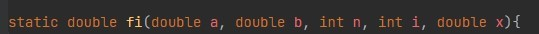
\includegraphics[scale=0.8]{error3.jpg}
            \caption{Użycie zwykłej zaproksymacji}
        \end{center}
    \end{figure}    

    \section{Źródła}
    \begin{enumerate}
        \item $https://pl.wikipedia.org/wiki/Wielomiany_Hermite'a$
    \end{enumerate}

\end{document}